% !TeX spellcheck = cs_CZ
%{\tikzset{external/prefix={tikz/FYZI/}}
% \tikzset{external/figure name/.add={ch06_}{}}
%---------------------------------------------------------------------------------------------------
% file fey1ch08.tex
%---------------------------------------------------------------------------------------------------
%================= Kapitola: Pohyb =================================================================
\setchaptertoc
\chapter{Pohyb}\label{fyz:IchapVIII}
  \luagraphic[1]{fyz_fig0908.jpg}{Human cannonball: Hugo Zacchini (20. října 1898 - 20. října 1975), 
                 jeden z bratrů Zacchini, byl první lidskou dělovou koulí, vystřelený kanónem 
                 na stlačený vzduch.}{fyz:fig0908}
  Cirkusové umění odjakživa přitahovalo pozornost diváků. Proto také bylo ve své době velmi
  rozšířené po celém světě a ve známých artistických rodinách se dědilo z generace na generaci. V
  roce 1922 užaslo obecenstvo nad číslem rodiny Zacchiniových, při kterém se jeden z nich nechal
  vystřelit z děla. Přeletěl celou cirkusovou arénu a dopadl do záchranné sítě. Divácky úspěšný
  kousek se v průběhu dalších let postupně zdokonaloval. Až nakonec, někdy kolem roku 1939 nebo
  1940, se podařilo Emanuelu Zacchiniovi překonat vzdálenost \qty{68.6}{\metre} a přeletět tři ruská
  kola v zábavním parku. Jak ale mohl vědět, kam je třeba umístit záchrannou síť? Kde získal
  jistotu, že dosáhne takové výšky, aby obrovská kola bez úhony přeletěl?

  \section{Popis pohybu}\label{fyz:IchapVIIIsecI}
      
    \begin{table}[ht!]      %\ref{fyz:tab002}
      \centering
      \renewcommand{\arraystretch}{1}
      \begin{tabular}{>{\centering\arraybackslash}p{3em}|>{\centering\arraybackslash}p{3em}}
        \hline \(t\)     & \(s\)          \\
        \([\text{min}]\) & \([\text{m}]\) \\
        \hline    \num{0} & \num{0}        \\
                  \num{1} & \num{360}      \\
                  \num{2} & \num{1200}     \\
                  \num{3} & \num{2700}     \\
                  \num{4} & \num{2850}     \\
                  \num{5} & \num{2880}     \\
                  \num{6} & \num{3900}     \\
                  \num{7} & \num{5400}     \\
                  \num{8} & \num{7050}     \\
                  \num{9} & \num{7200}     \\
        \hline 
      \end{tabular}
      \caption{Záznam automobilem ujeté vzdálenosti (\cite[s.~109]{Feynman01})}
      \label{fyz:tab002}
    \end{table}
    Abychom našli zákony, podle nichž probíhají změny s tělesy v průběhu času, musíme umět 
    \emph{popsat} tyto změny a nějakým způsobem je zaznamenat. Nejjednodušší změna, již je možno 
    pozorovat v případě tělesa, je zjevná změna jeho polohy s časem, a tu nazýváme pohybem. 
    Uvažujme nějaký tuhý předmět se stálou značkou, kterou nazveme bodem a kterou můžeme pozorovat. 
    Budeme si všímat pohybu této malé značky, jíž může být ozdoba na kapotě automobilu nebo střed 
    padající kuličky, a budeme se snažit popsat tu skutečnost, že se pohybuje a jakým způsobem se 
    to děje.

    Tyto příklady se možná zdají příliš jednoduché, ale popis změny zahrnuje mnoho detailů. Některé 
    změny jsou obtížněji popsatelné než pohyb bodu na tuhém tělese. Takovými jsou například pohyb 
    mraku, který nejenže pomalu postupuje, ale rychle mění svůj tvar, nebo se odpařuje a takové 
    jsou i vrtochy ženské mysli. Neznáme jednoduchý způsob analýzy změn mysli, ale mrak si můžeme 
    představit jako množství molekul, a tak snad v principu můžeme popsat pohyb mraku pomocí pohybu 
    jednotlivých molekul. Možná i změny v mysli jsou odrazem změn atomů v mozku, ale zatím o tom 
    nic nevíme.

    \begin{table}[ht!]       %\ref{fyz:tab003}
      \centering
      \renewcommand{\arraystretch}{1}
      \begin{tabular}{>{\centering\arraybackslash}p{2em}|>{\centering\arraybackslash}p{3em}}
        \hline  \(t\)    & \(s\)          \\
        \([\text{s}]\)   & \([\text{m}]\)   \\
         \hline  \num{0} & \num{0}          \\
                 \num{1} & \num{5}          \\
                 \num{2} & \num{20}         \\
                 \num{3} & \num{45}         \\
                 \num{4} & \num{80}         \\
                 \num{5} & \num{125}        \\
                 \num{6} & \num{180}        \\
        \hline 
      \end{tabular}
      \caption{Dráha padajícího míčku (\cite[s.~110]{Feynman01})}
      \label{fyz:tab003}
    \end{table}
    Začneme proto pozorovat pohyb bodů; můžeme je považovat za atomy, ale snad bude lepší, 
    budeme-li zpočátku méně přesní a budeme je považovat za nějaké malé předměty - malé v porovnání 
    se vzdálenostmi, na nichž se uskutečňuje pohyb. Například při popisu pohybu automobilu, který 
    ujel \qty{100}{\km}, nemusíme rozlišovat, jestli jde o přední nebo zadní nárazník. Máme-li být 
    přesní, jsou v tom drobné rozdíly, ale pro běžné účely stačí hovořit o „automobilu“ a nevadí 
    nám, že naše body nejsou skutečnými body - pro naše účely nemusíme být až tak přesní. Při 
    prvním pohledu na náš předmět zapomeneme i na trojrozměrnost světa. Soustředíme se jen na pohyb 
    v jednom směru, jako když jede automobil po silnici. Budeme-li vědět, jak popisovat 
    jednorozměrný pohyb, vrátíme se k trojrozměrnému prostoru. Jak je možné popsat takový 
    jednorozměrný pohyb - například pohyb auta? Nic nemůže být jednodušší. Z mnoha možných způsobů 
    vybereme následující. Abychom určili polohu auta v různých časových okamžicích, budeme měřit 
    jeho vzdálenost od počátečního bodu a zaznamenávat všechna pozorování. V tab. \ref{fyz:tab002} 
    představuje \(s\) vzdálenost auta od počátečního bodu v metrech a \(t\) představuje čas v 
    minutách.

    První řádek představuje nulovou vzdálenost a nulový čas - auto ještě neodstartovalo. Za jednu 
    minutu od startu ujelo \num{360} metrů.

    Po dvou minutách od startu se dostalo ještě dále - všimněte si, že větší vzdálenost ujelo v 
    druhé minutě-jeho pohyb se zrychlil. Mezi třetí a čtvrtou minutou se však něco stalo a v páté 
    minutě auto snad i zastavilo na červenou. Potom se jeho pohyb opět zrychlil a dostalo se do 
    vzdálenosti \num{3900} metrů na konci šesté minuty, do vzdálenosti \num{5400} metrů na konci 
    sedmé minuty, do vzdálenosti \num{7050} metrů na konci osmé minuty a v deváté minutě se dostalo 
    jen do vzdálenosti \num{7200} metrů, neboť ho zastavil policista.

    To je jeden způsob popisu pohybu. Druhým způsobem je popis pomocí grafu. Nanášíme-li čas 
    horizontálně a vzdálenost vertikálně, dostaneme křivku jako na obr. \ref{fyz:fig0098a}. S 
    rostoucím časem roste i vzdálenost, zpočátku velmi pomalu, potom rychleji a ve čtvrté minutě 
    opět velmi pomalu; potom několik minut roste a nakonec v deváté minutě přestane růst. Tyto 
    údaje je možno vyčíst z grafu bez použití tabulky. K úplnému popisu bychom samozřejmě 
    potřebovali i údaje o poloze auta při půlminutových značkách, ale zakreslujeme-li graf jako 
    spojitou křivku, děláme to proto, že předpokládáme, že auto i v mezičasech musí mít nějakou 
    polohu.
    
    Pohyb auta je složitý. Proto si za další příklad vybereme něco, co se pohybuje jednodušeji, co 
    vyhovuje jednodušším pohybovým zákonům - vybereme si padající míček. V tab. \ref{fyz:tab003} je 
    pro padající těleso čas vyjádřený v sekundách a vzdálenost v metrech. V nulté sekundě míček 
    začíná padat z nulové vzdálenosti a na konci první sekundy se dostal do vzdálenosti \num{5} 
    metrů. Na konci druhé sekundy je \num{20} metrů pod úrovní začátku, na konci třetí sekundy 
    \num{45} metrů atd. Vyneseme-li čísla z tabulky do grafu, získáme krásnou parabolu znázorněnou 
    na obr. \ref{fyz:fig0098b}, kterou je možné vyjádřit vztahem
    
    \begin{equation}\label{fyz:eq111}
      s = 5t^2.
    \end{equation}
  
    \begin{figure}[ht!]  %\ref{fyz:fig0098}
      \centering
      \subcaptionbox{\label{fyz:fig0098a}}{\luafigure[0.8]{fyz_fig0098a.pdf}}              \\                                                   
      \subcaptionbox{\label{fyz:fig0098b}}{\luafigure[0.8]{fyz_fig0098b.pdf}}
      \caption{a) Graf závislosti autem ujeté vzdálenosti na čase b) Časová závislost vzdálenosti 
               padajícího tělesa (\cite[s.~109]{Feynman01})}
      \label{fyz:fig0098}
    \end{figure}


    Tento vztah nám umožňuje vypočítat vzdálenost v kterémkoli časovém okamžiku. Snad namítneme, že 
    by měl existovat vztah i pro první graf. Takový vztah je možné zapsat obecně ve tvaru
    \begin{equation}\label{fyz:eq112}
      s = f(t),
    \end{equation}
    což znamená, že \(s\) je veličinou, která závisí na \(t\), nebo v matematickém jazyku je \(s\) 
    funkcí \(t\). Protože nevíme, jaká ta funkce je, nemůžeme ji vyjádřit v konkrétním algebraickém 
    tvaru.

    Poznali jsme dva příklady pohybu jež byly popsány velmi jednoduchým způsobem bez zvláštní 
    důmyslnosti. Avšak tyto příklady v sobě přece jen skrývají několik jemností. Především, co 
    rozumíme časem a prostorem? Ukazuje se, že jde o hluboké filozofické otázky, jež si ve fyzice 
    vyžadují důkladnou analýzu a ta nebývá snadná. Teorie relativity ukazuje, že představy prostoru 
    a času nejsou tak jednoduché, jak by se zdály na první pohled. Jenže zatím v našich prvních 
    úvahách nemusíme být příliš úzkostliví při definování těchto pojmů. Některým z nás se to bude 
    zdát divné, neboť jsme se učili, že ve vědě je třeba \emph{vše} přesně definovat. Jenže 
    \emph{vše} přesně definovat nemůžeme! Kdybychom se o to pokusili, dostali bychom se do podobné 
    situace jako ti dva filozofové, kteří v diskusi říkají jeden druhému: „Sám nevíte, o čem 
    hovoříte!“ Druhý odpovídá; ,A co to znamená \emph{vědět}? Co znamená \emph{hovořit}? Co znamená 
    \emph{sáni}?“ Abychom mohli hovořit konstruktivně, musíme se dohodnout, že mluvíme zhruba o 
    stejné věci. O čase už víme vše, co teď potřebujeme. Musíme si však být vědomi toho, že 
    existuje řada detailů, jež bude třeba prodiskutovat, ale to uděláme až později.
    
    Jednou z takových diskutabilních věcí je již uvedený fakt, že pozorovaný pohybující se bod se 
    vždy nachází na nějakém místě. (Samozřejmě, když na něj hledíme, je tam, ale bude tam i tehdy, 
    kdy se na něj nedíváme?) Ukazuje se, že v případě pohybujících se atomů není možné takto 
    uvažovat - na atomu si nemůžeme zvolit značku a pozorovat její pohyb. S tímto problémem se 
    setkáme v kvantové mechanice. Nejprve se však budeme zajímat o problémy, v nichž ještě 
    neuvažujeme takové komplikace, a až \emph{později} provedeme korekce, které si vynucují 
    nejnovější poznatky. Uspokojíme se proto s jednoduchým pohledem na čas a prostor. Víme, co tyto 
    pojmy v hrubých rysech představují a ti, kteří již řídili auto, vědí, co znamená rychlost.
    
  \section{Rychlost}
    Ačkoli zhruba víme, co „rychlost“ znamená, přece tu existují určité rafinované záludnosti; 
    vždyť jen uvažme, že učení Řekové nebyli schopni přiměřeně popsat problémy související s 
    rychlostí. Taková záludnost se objeví, když se snažíme přesně pochopit, co je třeba rozumět pod 
    „rychlostí“. Řekové z toho byli velmi zmateni a muselo být objeveno nové odvětví matematiky 
    (vedle geometrie a algebry Řeků, Arabů a Babylóňanů). Pro ilustraci problémů se pokusme řešit 
    tento problém jednoduchou algebrou: Balón nafukujeme tak, že jeho objem roste rychlostí 
    \qty{100}{\cubic\cm} za sekundu; jakou rychlostí roste jeho poloměr, když má balón 
    \qty{1000}{\cubic\cm}? Řeky jaksi zmátl takovýto problém zejména zásluhou některých úmyslně 
    matoucích Řeků. Aby poukázal na těžkosti související se studiem rychlosti, Zenon uvedl několik 
    paradoxů, ze kterých uvedeme jeden pro ilustraci problémů, jež se vyskytly při zkoumání pohybu. 
    V tomto paradoxu Zenon říká, že Achilles, ačkoli běží l0krát rychleji než želva, přece ji nikdy 
    nedoběhne. Argumentuje následujícím způsobem: „Předpokládáme-li, že na začátku běhu má želva 
    stometrový náskok, pak než Achilles uběhne \num{100} metrů a dostane se na místo, kde byla 
    původně želva, bude želva, která leze desetkrát pomaleji, \num{10} metrů před ním. Achilles 
    proto musí běžet dalších \num{10} metrů, aby želvu chytil, ale po deseti metrech zjistí, že 
    želva je \num{1} metr před ním. Když uběhne i ten metr, najde želvu \qty{10}{\cm} před sebou a 
    tak to půjde \emph{donekonečna}. Proto je v kterémkoli okamžiku želva před Achillem a ten ji 
    nikdy nedoběhne“. Co je na této argumentaci nesprávné? Je to skutečnost, že konečný čas se dělí 
    na nekonečně mnoho částí, právě tak jako konečná délka se dá rozdělit na nekonečně mnoho částí 
    opakovaným dělením dvěma. A tak, ačkoli (při této argumentaci) máme nekonečný počet kroků k 
    bodu, v němž Achilles dostihne želvu, neznamená to, že jde o nekonečně dlouhý \emph{časový} 
    interval. Na tomto příkladu je vidět, že při studiu rychlosti je možné narazit na problémy.
    
    Abychom si mohli ještě jasněji představit tyto problémy, připomeňme vtip o autě, které zastavil 
    policista. Nyní si představme, že v tomto autě sedí dáma a policista ji napomíná: „Paní, jela 
    jste rychlostí \num{90} km za hodinu!“ Dáma odpovídá: „To přece není možné, vždyť cestuji jen 
    sedm minut! Je to směšné -jak mohu jet rychlostí \num{90} km za hodinu, když jsem hodinu 
    nejela?“ Jak bychom odpověděli, kdybychom byli policistou? Samozřejmě, kdybychom skutečně byli 
    policistou, vše by bylo bez problémů. Prostě bychom té dámě řekli, že svoje argumenty může 
    přednést u soudu. Vyloučíme-li však takové řešení a uspokojíme se s poctivým intelektuálním 
    přístupem k tomuto problému, v němž chceme této dámě vysvětlit, co znamená jet rychlostí 
    \num{90} km za hodinu, co musíme udělat? Té dámě bychom vysvětlili, že kdyby pokračovala v 
    cestě a jela stále stejnou rychlostí, ujela by za hodinu \num{90} kilometrů. Mohla by však 
    namítnout: „Dala jsem nohu z plynu a auto zpomalovalo, a proto bych neujela \num{90} km, 
    kdybych takto pokračovala.“ Nebo uvažujme padající míček a předpokládejme, že bychom chtěli 
    znát jeho rychlost za dobu tří sekund, kdyby se dále pohyboval tak, jak se pohybuje nyní. 
    Znamenalo by to snad, že si udržuje \emph{zrychlení} a pohybuje se stále rychleji? Ne, 
    znamenalo by to, že si udržuje stejnou \emph{rychlost}. A to právě chceme definovat! Kdyby 
    totiž míček setrvával v původním pohybu, pohyboval by se tak, jak se pohybuje. Rychlost proto 
    musíme lépe definovat. Co se má vlastně zachovat? Ta dáma by také mohla argumentovat 
    následujícím způsobem: „Kdybych pokračovala v pohybu bez změny další hodinu, narazila bych do 
    zdi na konci ulice!“ Není tedy tak jednoduché říci, co vlastně máme na mysli.
    
    Mnozí fyzici zastávají názor, že měření je jedinou definicí kterékoli veličiny. Pak bychom, 
    samozřejmě, použili zařízení na měření rychlosti - \textbf{tachometr} - a upozornili bychom 
    dámu, že její tachometr ukazuje \num{90}. Dáma by však opět mohla namítat, že její tachometr je 
    pokažený a vůbec neukazuje. Znamená to ale, že se auto nepohybuje? Jsme přesvědčeni, že 
    existuje něco, čím je možné změřit rychlost dříve, než zkonstruujeme tachometr. Jen tehdy je 
    možné říci například: „Tachometr nepracuje správně“ nebo „tachometr je rozbitý“. Kdyby nebylo 
    možné měřit rychlost jinak než tachometrem, byla by tato věta nesmyslem. Máme tedy na mysli 
    něco, co je nezávislé na tachometru a tachometr slouží jen k měření této myšlenky. Uvažme, zda 
    je možné lépe definovat rychlost. Jako policista bychom řekli: „Milá paní, kdybyste jela 
    hodinu, narazila byste na zeď, ale kdybyste jela jednu sekundu, ujela byste \num{25} metrů. 
    Jela jste tedy rychlostí \num{25} metrů za sekundu a další sekundu byste ujela dalších \num{25} 
    metrů a ta zeď je mnohem dále.“ Dáma však namítá: „Neexistuje ale takový zákon, který by říkal, 
    že není dovoleno jet \num{25} metrů za sekundu! Zákon zakazuje jet \num{90} km za hodinu.“ Vy 
    potom řeknete, že je to přece totéž. Je-li to však totéž, pak by asi nedošlo k takové tahanici 
    o \num{25} metrů za sekundu. Padající míček se ve skutečnosti nemůže pohybovat stejně v průběhu 
    ani jedné sekundy, protože stále mění rychlost, a tak budeme muset rychlost nějak definovat.
    
    Zdá se, že se dostáváme na správnou stopu. Kdyby dáma pokračovala v cestě další tisícinu 
    hodiny, ujela by tisícinu z \num{90} km. Jinými slovy: nemusela by jet celou hodinu, důležité 
    je, že v \emph{daném okamžiku} jede takovou rychlostí. To znamená, že kdyby jela jen o nepatrný 
    okamžik déle, ujela by navíc takový úsek, jaký by ujelo auto jedoucí \emph{stálou} rychlostí 
    \num{90} km za hodinu. Myšlenka o \num{25} metrech za sekunduje možná správná; sledujeme, kolik 
    auto ujelo za poslední sekundu, dělíme to \num{25} metry a když dostaneme \num{1}, rychlost 
    byla \num{90} km za hodinu. Jinými slovy, rychlost můžeme zjistit tímto způsobem: zjistíme, jak 
    daleko dojdeme ve velmi krátkém čase, pak tuto vzdálenost dělíme časem, a tak dostaneme 
    rychlost. Čas je však třeba zvolit co nejkratší, neboť v průběhu tohoto času by se mohla stát 
    nějaká změna. Kdybychom v případě padajícího tělesa zvolili za takový časový interval hodinu, 
    bylo by to absurdní. Kdybychom zvolili jednu sekundu, dostali bychom docela dobrý výsledek v 
    případě auta, kdy je změna rychlosti malá, ale taková volba by nebyla dostatečná pro padající 
    těleso. Chceme-li zjistit rychlost co nejpřesněji, musíme zvolit časový interval co nejkratší. 
    Měli bychom tedy zvolit milióntinu sekundy a vzdálenost ujetou za tento čas dělit tou 
    milióntinou sekundy. Tak bychom dostali vzdálenost za sekundu, neboli to, co rozumíme jako 
    rychlost a takovýmto způsobem vlastně definujeme rychlost. Takto by bylo třeba odpovědět dámě v 
    automobilu, taková je definice, kterou budeme používat.
    
    Definice rychlosti obsahuje novou myšlenku, jež ve své obe\-cné podobě nebyla dostupná starým 
    Řekům. Tato myšlenka spočívá v tom, že uvažujeme \emph{nekonečné malou vzdálenost} a 
    odpovídající \emph{nekonečné malý čas}, uvedeme je do poměru a sledujeme chování tohoto poměru 
    při zmenšování časového intervalu. Jinak řečeno, zajímáme se o \textbf{limitu} ujeté 
    vzdálenosti dělenou odpovídajícím časem při \emph{nekonečném} zmenšování tohoto času. Na tuto 
    myšlenku přišli nezávisle na sobě Newton a Leibniz a představovala zrod nové matematické 
    disciplíny nazývané \textbf{diferenciální počet}. Tento počet vznikl v souvislosti s popisem 
    pohybu a jeho první aplikací byl vlastně náš problém související s otázkou: Co znamená jet 
    \uv{90 km/hod}?

    Pokusme se definovat rychlost trochu přesněji. Předpokládejme, že za krátkou dobu 
    \(\varepsilon\) urazí auto nebo jiné těleso krátkou vzdálenost \(x\). Pak definujeme rychlost 
    \(v\) jako
    \begin{equation}\label{fyz:eq113}
      v = \frac{x}{\varepsilon}.
    \end{equation}
    přičemž přesnost bude tím větší, čím bude \(\varepsilon\) menší. Chceme-li to vyjádřit 
    matematicky, můžeme říci, že rychlost je limita podílu \(x/\varepsilon\) při \(\varepsilon\) 
    blížícím se k nule, tj.
    \begin{equation}\label{fyz:eq114}
      v = \lim_{\varepsilon\to 0}{\frac{x}{\varepsilon}}.
    \end{equation}
    
    V případě dámy s autem nemůžeme provést totéž, neboť naše tabulka je neúplná. Víme jen to, kde 
    se dáma nachází na hranicích minutových intervalů. Proto si můžeme vytvořit jen přibližný obraz 
    o její rychlosti z toho, že například po dobu sedmé minuty ujela \num{1500} metrů, ale nevíme, 
    jaká byla její rychlost přesně na začátku sedmé minuty. Nevíme, zda zrychlovala a na začátku 
    šesté minuty měla rychlost \qty{1400}{\m/\min} a nyní má rychlost \qty{1600}{\m/\min}, nebo zda 
    pohyb probíhal jinak. Nevíme to proto, že nám chybí údaje uvnitř intervalu. Z takové tabulky 
    bychom mohli vypočítat rychlost jen tehdy, kdyby obsahovala nekonečně mnoho údajů. Máme-li však 
    matematický vztah úplný - takovým je v případě padajícího tělesa rovnice (\ref{fyz:eq111}) - 
    můžeme vypočítat takovouto rychlost, neboť umíme určit polohu tělesa v kterémkoli časovém 
    okamžiku.
    
    Jako příklad si určíme rychlost padajícího tělesa v páté sekundě pádu. Jedním ze způsobů jak to 
    provést by mohlo být zkoumání \emph{tabulky} \ref{fyz:tab003}, z níž je vidět, že v páté 
    sekundě urazilo těleso \(125 - 80 = \qty{45}{\m}\). Proto by se zdálo, že těleso padalo 
    rychlostí \qty{45}{\m/\s}. To však není pravda, neboť rychlost se mění a ačkoli v tomto časovém 
    intervalu je to \emph{y průměru \qty{45}{\m/\s}}, těleso se zrychluje a na konci páté sekundy 
    padá rychleji než \qty{45}{\m/\s}. Chceme \emph{přesné určit jeho rychlost}. Je možné to udělat 
    následujícím způsobem: Víme, kde se těleso nacházelo v páté sekundě. V \qty{5.1}{\s} je podle 
    vztahu (\ref{fyz:eq111}) vzdálenost, kterou těleso urazilo, rovna \(5\cdot5,1^2 = \qty{130.05} 
    {\m}\). V páté sekundě bylo těleso ve vzdálenosti \qty{125}{\m} a za další desetinu sekundy 
    urazilo \(\num{130.05} - \num{125} = \qty{5.05}{\m}\). Protože \qty{5.05}{\m} za \qty{0.1}{\s} je 
    totéž jako \qty{5.05}{\m\per\s}, zjistili jsme vlastně rychlost, ale ne zcela přesně. Nevíme, 
    je-li to rychlost v páté sekundě, v \qty{5.1}{\s} nebo \qty{5.05}{\s}, nebo někde mezi těmito 
    hodnotami. Měli jsme určit rychlost v \qty{5}{\s} a jestliže se nám to zcela nepodařilo, 
    zpřesníme náš postup. Vezmeme jednu tisícinu sekundy a vypočítáme, kam se až dostalo těleso. 
    Přidáme-li ještě tento čas k páté sekundě, dostaneme tedy v \qty{5.001}{\s}
    \begin{equation*}
      s = 5\cdot5,001^2 = 5\cdot25,010001 = \qty{125.050005}{\m}.
    \end{equation*}
    
    V poslední tisícině sekundy spadlo těleso \qty{0.050005}{\m} a dělíme-li toto číslo 
    \qty{0.001}{\s}, dostaneme rychlost \qty{50.005}{\m/\s}. Tento údaj je již přesnější, již je 
    docela blízký skutečnosti, ale přece jen není zcela přesný. Je však vidět, co musíme udělat, 
    chceme-li rychlost určit přesně. Bude užitečné formulovat úlohu trochu abstraktněji: Hledáme 
    rychlost v časovém okamžiku \(t_0\) Jenž v našem původním problému představoval \qty{5}{\s}. 
    Vzdálenost, do níž se dostalo těleso v čase \(t_0\) a kterou budeme označovat \(s_0\), je rovna 
    \(5t_0^2\) , tedy \qty{125}{\m} v našem případě. Při hledání rychlosti si klademe otázku: 
    \uv{Kde je těleso v čase \(t_{0+}\) (malý přírůstek) nebo \(t_0 + \varepsilon\)?} Nová poloha 
    je \(5(t_0 + \varepsilon)^2 = 5t_0^2 + 10t_0\varepsilon + 5\varepsilon^2\). Těleso je teď dále 
    než předtím, neboť nejprve bylo vzdáleno jen \(5t_0^2\) . Ta dodatečná vzdálenost je \(s_{0+}\) 
    (malý přírůstek) nebo \(s_0 + x\) (kde \(x\) je ten přírůstek). Odečteme-li od vzdálenosti 
    v čase \(t_0 + \varepsilon\) vzdálenost v \(t_0\), dostaneme \(x\) - přírůstek vzdálenosti jako 
    \(x = 10t_0\varepsilon +5\varepsilon^2\). V prvním přiblížení bude rychlost rovna
    \begin{equation}\label{fyz:eq116}
      v = \frac{x}{\varepsilon} = 10t_0 +5\varepsilon.
    \end{equation}
    
    Skutečná rychlost je hodnota tohoto poměru \(x/\varepsilon\) při nepatrném \(\varepsilon\). 
    Jinými slovy, po vytvoření poměru bereme \(\varepsilon\) vždy menší a menší, tj. blížící se k 
    nule. Rovnice pak přejde do tvaru \(v\)(v čase \(t_0\)) = \(10t_0\). V našem případě bylo \(t_0 
    = \qty{5}{\s}\), a proto \(v = 10\cdot5 = \qty{50}{\m/\s}\). Předtím, když jsme uvažovali 
    \(\varepsilon\) nejprve \qty{0.1}{\s} a podruhé \qty{0.001}{\s}, byla hodnota \(v\) trochu větší. 
    Nyní však vidíme, že skutečná rychlost je přesně \qty{50}{\m/\s}.
    
  \section{Rychlost jako derivace}
    Výpočet, který jsme právě provedli, je v matematice velmi častý a pro veličiny \(\varepsilon\) 
    a \(x\) se proto zavedlo speciální značení: Namísto \(\varepsilon\) se setkáme s \(\Delta t\) a 
    namísto \(x\) s \(\Delta s\). Pod \(\Delta t\) rozumíme \uv{malý přírůstek \(t\)}, který je 
    možné vždy zmenšovat. Přítomnost znaku \(\Delta\) neznamená násobení, právě tak jako 
    \(\sin\vartheta\) neznamená \(s\cdot i \cdot n \cdot \vartheta\). Jde prostě o časový přírůstek 
    a znak \(\Delta\) zvýrazňuje jeho zvláštní charakter. Podobnou vlastnost má \(\Delta s\), 
    rozdíl je jen v tom, že tentokrát jde o vzdálenost \(s\). Protože \(\Delta\) není součinitel, 
    nevykrátí se v poměru \(\Delta s/\Delta t\) a nedostaneme \(s/t\), právě tak, jako bychom 
    nedostali \(1/2\) z výrazu \(\sin \vartheta/\sin2\vartheta\). Při takovémto značení je 
    \emph{rychlost rovna limitě podílu \(\Delta s/\Delta t\) při \(\Delta t\) blížícím se k nule}, 
    tedy
    \begin{equation}\label{fyz:eq117}
      \boxed{v = \lim_{\Delta t\to 0}{\frac{\Delta s}{\Delta t}}}\,.
    \end{equation}
    Tento výraz je stejný, jako vztah (\ref{fyz:eq114}) s \(\varepsilon\) a \(x\), ale má tu 
    výhodu, že poukazuje na změnu určitých veličin a ukazuje co a jak se mění.
    
    Existuje ještě jeden zákon, který platí s dostatečnou přesností. Ten zákon říká, že vzdálenost 
    pohybujícího se bodu je možné vyjádřit jako součin rychlosti a časového intervalu, tj. \(\Delta 
    s = v\Delta t\). Tento zákon je správný tehdy, když se v průběhu uvažovaného časového intervalu 
    rychlost nemění, ale to obecně platí jen tehdy, kdy je \(\Delta t\) dostatečně malé. Fyzici 
    jsou zvyklí psát \(\dd{s} = v\dd{t}\), přičemž pod \(\dd{t}\) rozumějí \(\Delta t\) za 
    podmínek, v nichž je velmi malé. Při takovémto chápání je uvedený zákon dostatečně přesný. 
    Kdyby \(\Delta t\) bylo velké, mohla by se rychlost v průběhu tohoto intervalu měnit a přesnost 
    zákona by se zmenšila. Při \(\dd{t}\) blížícím se k nule je výraz \(\dd{s} = v\dd{t}\) zcela 
    přesný. Pomocí nově zavedených symbolů můžeme vztah (\ref{fyz:eq117}) přepsat do tvaru
    \begin{equation}\label{fyz:eq118}
      v = \lim_{\Delta t\to 0}{\frac{\Delta s}{\Delta t}} = \der{s}{t}.
    \end{equation}
    
    Veličina \(ds/dt\) se v tomto vztahu nazývá \uv{derivace s podle \(t\)} (takový název nám 
    připomíná, co se vlastně mění) a složitý proces hledání derivace se nazývá derivováním. 
    Objevují-li se \(ds\), \(dt\) samostatně, nazývají se \textbf{diferenciály}. Aby se nám stala 
    nová řeč bližší, připomeňme si, že již dříve jsme počítali derivaci funkce \(5t^2\), o níž jsme 
    zjistili, že je rovna \(10t\). Zvykneme-li si na novou řeč, budeme snadněji chápat mnohé 
    myšlenky. Abychom se pocvičili, vypočítáme derivaci složitější fimkce. Uvažujme vztah \(s = 
    At^3 + Bt+ C\), jenž by mohl popisovat pohyb bodu. Písmena \(A\), \(B\), \(C\), podobně jako ve 
    známém obecném tvaru kvadratické rovnice, představují konstantní čísla. Naším úkolem je najít 
    rychlost v kterémkoli okamžiku na základě tohoto vztahu. Abychom to provedli co nejelegantněji, 
    změníme \(t\) na \(t + \Delta t\), přičemž se změní \(s\) na \(s + \Delta s\) a \(\Delta s\) 
    vyjádříme pomocí \(\Delta t\) Tak dostaneme
    \begin{align}\label{fyz:eq119}
     s + \Delta s &= A(t + \Delta t)^3 + B(t + \Delta t) + C    \nonumber \\
                  &= At^3 + Bt + C + 3At^2\Delta t + B\Delta t  \nonumber \\
                  &+ 3At(\Delta t)^2 + A(\Delta t)^3.
    \end{align}
    Protože \(s = At^3 + Bt + C\), můžeme psát
    \begin{equation}\label{fyz:eq120}
         \Delta s = 3At^2\Delta t + B\Delta t + 3At(\Delta t)^2 + A(\Delta t)^3.
    \end{equation}

    \begin{table}      %\ref{fyz:tab005}
      \resizebox{1\linewidth}{!}{
      \renewcommand{\arraystretch}{1.0} 
      \noindent\begin{tabular*}{\columnwidth}{@{\extracolsep{\stretch{1}}}*{2}{l}@{}}
        \toprule
        \small Funkce & \small Derivace \(\der{s}{t}\)\\
        \midrule
        \(s = t^n\)             & \(nt^{n-1}\)                                                   \\
        \(s=cu\)                & \(c\der{u}{t}\)                                                \\
        \(s = u+v+w+\ldots\)    & \(\der{u}{t} + \der{v}{t} + \der{w}{t} + \ldots\)              \\
        \(s = c\)               & \(0\)                                                          \\
        \(s = u^av^bw^c\ldots\) & \(s\left(\frac{a}{u}\der{u}{t} + 
                                  \frac{b}{v}\der{v}{t} + \frac{c}{w}\der{w}{t} +\ldots\right)\) \\
        \bottomrule 
      \end{tabular*}
      }
      \caption{Stručný přehled derivací: \(s\), \(u\), \(v\), \(w\) jsou libovolné funkce; \(t\), 
               \(a\), \(b\), \(c\), \(n\) jsou libovolné konstanty  
               (\cite[s.~114]{Feynman01})}
      \label{fyz:tab005}
    \end{table}
    
    Jenže my nepotřebujeme \(\Delta s\), ale \(\Delta s\) dělené \(\Delta t\). Proto předcházející 
    rovnici dělíme \(\Delta t\) a dostáváme
    \begin{equation}\label{fyz:eq121}
       \frac{\Delta s}{\Delta t} = 3At^2 + B + 3At(\Delta t) + A(\Delta t)^2.
    \end{equation}
    Jde-li \(\Delta t\) k nule, je \(\frac{\Delta s}{\Delta t}\) rovno \(\der{s}{t}\) a platí
    \begin{equation}\label{fyz:eq122}
       \frac{\Delta s}{\Delta t} = 3At^2 + B.
    \end{equation}
    
    To je základ derivování funkcí. Tento proces je ve skutečnosti ještě jednodušší, než by se na 
    první pohled zdálo. Všimněme si, že členy obsahující druhou nebo vyšší mocniny \(\Delta t\) je 
    možné zanedbat, neboť v limitě konvergují k nule.
    
    Po krátkém cvičení se celý proces pro nás stane ještě jednodušším, neboť budeme vědět, co je 
    třeba zanedbat. Existuje velmi mnoho pravidel derivování různých druhů funkcí. Tato pravidla je 
    možné si pamatovat, nebo je možné je vyhledat v tabulkách. Stručný seznam pravidel je uveden v 
    tab. \ref{fyz:tab005}.
  
  \section{Vzdálenost jako integrál}
    \begin{table}[ht!]        %\ref{fyz:tab004}
      \centering
      \renewcommand{\arraystretch}{1.0}
      \begin{tabular}{>{\centering\arraybackslash}p{2em}|>{\centering\arraybackslash}p{3em}}
        \hline  \(t\)    & \(v\)          \\
                 \unit{\s} & \unit{\m\per\s}  \\
         \hline  \num{0} & \num{0}        \\
                 \num{1} & \num{10}       \\
                 \num{2} & \num{20}       \\
                 \num{3} & \num{30}       \\
                 \num{4} & \num{40}       \\
        \hline 
      \end{tabular}
      \caption{Rychlost padajícího tělesa (\cite[s.~115]{Feynman01})}
      \label{fyz:tab004}
    \end{table}
    Ještě nám zbývá analyzovat obrácenou úlohu. Předpokládejme, že místo tabulky vzdáleností máme 
    tabulku rychlostí v různých časech počínaje nulou. Pro padající kuličku jsou tyto rychlosti a 
    časy znázorněny v tab. \ref{fyz:tab004}. Podobnou tabulku je možné sestavit pro auto, 
    zaznamenáváme-li údaje tachometru každou minutu nebo každou půlminutu. Víme-li v každém časovém 
    okamžiku, jak rychle se auto pohybuje, můžeme určit, jak daleko se dostane? Tato úloha je 
    opakem úlohy, kterou jsme již vyřešili; je dána rychlost a chceme určit vzdálenost. Jak je 
    možné určit vzdálenost, známe-li rychlost? Není-li rychlost auta konstantní a dáma se chvíli 
    pohybuje rychlostí \qty{90}{\km\per\hour}, pak zpomalí, opět zrychlí atd., jak můžeme určit, kam 
    se až dostala? Je to jednoduché. Použijeme stejnou myšlenku jako v předcházejícím případě a 
    vyjádříme vzdálenost pomocí nekonečně malých částí. Jestliže mělo auto v první sekundě určitou 
    rychlost, můžeme ze vztahu \(\Delta s = v\Delta t\) vypočítat, kam až se auto při dané 
    rychlosti v první sekundě dostalo. V další sekundě se rychlost auta liší o málo; kam se auto 
    dostalo, vypočítáme tak, že vynásobíme novou rychlost časem. Takto dostáváme jistý počet malých 
    vzdáleností a celková vzdálenost bude součtem těchto malých vzdáleností. To znamená, že 
    vzdálenost bude součtem součinů rychlostí a časů, tedy \(s=\sum v\Delta t\), kde řecké písmeno 
    \(\sum\) (sigma) označuje součet. Pro přesnost je třeba poznamenat, že v součtu vystupují 
    rychlosti v určitém okamžiku, např. \(i\)-tém časovém okamžiku a jsou násobeny \(\Delta t\), tj.
    \begin{equation}\label{fyz:eq123}
      s = \sum_{i}v(t_i)\Delta t.
    \end{equation}
    Tyto časové okamžiky vyhovují následující podmínce: \(t_{i+1} = t_i + \Delta t\). Ani takovémto 
    způsobem určovaná vzdálenost nebude přesná, neboť v průběhu časového intervalu \(\Delta t\) se 
    může rychlost měnit. K zabezpečení přesnosti musíme časové intervaly brát co nejkratší. 
    Skutečné \(s\) je
    \begin{equation}\label{fyz:eq124}
      s = \lim_{\Delta t\to0}\sum_{i}v(t_i)\Delta t.
    \end{equation}
    Pro takovouto limitu zavedli matematici speciální symbol analogický symbolu pro diferenciál.    
    \(\Delta\) přechází v \(d\) a zvýrazňuje tak skutečnost, že čas je co nejmenší, o rychlosti 
    hovoříme jako o \(v\) v čase \(t\) a součet píšeme s trochu deformovaným velkým „S“ \(\int\) 
    (podle latinského slova \emph{summa}), kterému se dnes říká bohužel jen znak integrálu. Máme 
    tedy
    \begin{equation}\label{fyz:eq125}
      \boxed{s = \int\sum_{i}v(t_i)\Delta t}\,.
    \end{equation}
    
    Proces sčítání takových výrazů se nazývá \textbf{integrování} a představuje \emph{opak} 
    derivování. Derivace tohoto integrálu je \(v\), takže jeden operátor (\(d\)) ruší druhý 
    (\(\int\)). Vzorce pro integrování je možné získat ze vzorců pro derivování jejich obrácením, 
    neboť jsou vzájemně inverzní. Každý si může sestavit svou tabulku integrálů, bude-li derivovat 
    všechny druhy funkcí. Z každého diferenciálního vzorce dostaneme integrální, když ho obrátíme.
    
    Každou funkci je možné derivovat analyticky, tj. operace probíhá algebraicky a vede k určité 
    funkci. S integrálem je to však jinak a není možné napsat analytický tvar pro libovolný 
    integrál. Je sice možné ho vypočítat, například tak, že nejprve provedeme uvedenou sumaci, a 
    zjemníme-li dostatečně interval \(\Delta t\), dostaneme výsledek téměř přesně. Máme-li však 
    danou určitou funkci, nemůžeme obecně nalézt analytický výraz pro její integrál. Vždy se můžeme 
    pokusit najít funkci, která nám po zderivování dá požadovanou funkci. Jenomže taková funkce 
    nemusí existovat v tom smyslu, že by se dala vyjádřit pomocí funkcí, které již dostaly nějaké 
    pojmenování.
    
  \section{Zrychlení}
    Dalším krokem na cestě k pohybovým rovnicím je zavedení veličiny, která přesahuje pojem 
    rychlosti a souvisí se \emph{změnou} rychlosti pohybu. K takovéto veličině přicházíme, když si 
    klademe otázku, jak se \emph{mění} rychlost. V předcházejících kapitolách jsme hovořili o 
    případech, v nichž síly způsobovaly změny rychlosti. Určitě jsme již slyšeli vzrušující zprávy 
    o autech, která za \num{10} sekund dosáhnou z klidu rychlosti \qty{100}{km\per\hour}. Na 
    takovémto příkladu je vidět, jak se mění rychlost - ale jen v průměru. V dalším stádiu se 
    budeme zabývat složitějším problémem - rychlostí změny rychlosti. Jinými slovy, o kolik metrů 
    za sekundu se změní rychlost v průběhu sekundy, tj. o kolik metrů za sekundu za sekundu. Již 
    dříve jsme odvodili vztah pro rychlost padajícího tělesa v podobě \(v= 10 t\), který je 
    zaznamenán v tab. \ref{fyz:tab004}, a nyní bychom chtěli zjistit, jak se rychlost mění za 
    sekundu. Veličinu vyjadřující tuto změnu nazýváme \textbf{zrychlením}.
    
    Zrychlení je definováno jako časová změna rychlosti. Z předcházející diskuze již víme dost k 
    tomu, abychom mohli zapsat zrychlení jako derivaci \(\der{v}{t}\), podobně, jako rychlost byla 
    časovou derivací vzdálenosti. Derivujeme-li vztah \(v= 10t\), dostaneme zrychlení padajícího 
    tělesa
    \begin{equation}\label{fyz:eq101}
      a = \der{v}{t} = 10.
    \end{equation}
    
    (Při derivování výrazu \(10t\)l jsme využili výsledek získaný v předcházející úloze, kde jsme 
    zjistili, že derivace \(Bt\) je prostě \(B\) tedy konstanta. Položením \(B=10\) dostaneme 
    okamžitě výsledek, že derivace \(10t\) je \num{10}) To znamená, že rychlost padajícího tělesa 
    roste každou sekundu o \qty{10}{\m\per\s}. Tato skutečnost je zřejmá i z tab. 8.4. Tento příklad 
    je velmi jednoduchý, ale zrychlení obecně nebývají konstantní. Příčinou konstantního zrychlení 
    v případě padajícího tělesa je skutečnost, že na něj působí konstantní síla a podle Newtonova 
    zákona je zrychlení úměrné síle.
    
    Jako další příklad si všimněme zrychlení v úloze, kterou jsme již vyřešili, když jsme se 
    zabývali rychlostí. Když jsme vycházeli ze vztahu \(s = At^3 + Bt + C\), dostali jsme pro 
    \(v=\der{s}{t}\) vyjádření
    \begin{equation}\label{fyz:eq102}
      v = 3At^2 + B.
    \end{equation}
    
    Protože zrychlení je časová derivace rychlosti, musíme poslední výraz derivovat. Připomeňme si 
    pravidlo, podle něhož je derivace dvojčlenu rovna součtu derivací jednotlivých členů. Abychom 
    při derivování prvního členu nemuseli opakovat celý základní proces, připomeňme si, že 
    kvadratický člen jsme již derivovali při derivování funkce a výsledek byl takový, že koeficient 
    se zdvojnásobil a t2 se změnilo na t. Proto budeme předpokládat, že totéž se děje i v tomto 
    případě. Derivace \(3At^2\) proto bude \(6At\). Dále musíme derivovat \(B\), tedy konstantní 
    člen. Podle předcházejícího pravidla je však derivace \(B\) rovna nule, a tak tento člen 
    nepřispívá ke zrychlení. Konečný výsledek je proto \(a=\der{v}{t}= 6At\).
    
    Uveďme ještě dva užitečné vztahy, jež je možné získat integrací. Pohybuje-li se těleso 
    vycházející z klidu s konstantním zrychlením \(g\), jeho rychlost v libovolném čase \(t\) je
    \begin{equation}\label{fyz:eq103}
      v = gt.
    \end{equation}
    Vzdálenost, kterou těleso až do tohoto okamžiku urazí, je
    \begin{equation}\label{fyz:eq104}
      v = \frac{1}{2}gt^2.
    \end{equation}
    
    Pro zápis derivace se používají různá matematická značení. Protože rychlost je \(ds/dt\) a 
    zrychlení je časová derivace rychlosti, můžeme psát i
    \begin{equation}\label{fyz:eq105}
      a = \der{ }{t}\left(\der{s}{t}\right) = \dder{s}{t},
    \end{equation}
    což představuje běžný zápis druhé derivace.
    
    Existuje i jiný zákon, podle něhož je rychlost rovna integrálu zrychlení. To je právě opakem 
    vztahu \(a = \der{v}{t}\). Protože jsme již zjistili, že vzdálenost je integrálem rychlosti, 
    můžeme vzdálenost najít \emph{dvojnásobnou integrací zrychlení}.
    
    \begin{figure}[ht!]  %\ref{fyz:fig0099}
      \centering
      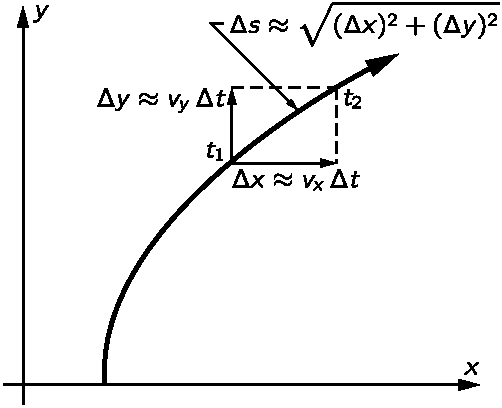
\includegraphics[width=0.8\linewidth]{fyz_fig0099.pdf}
      \caption{Popis pohybu tělesa v rovině a výpočet jeho rychlosti
               (\cite[s.~118]{Feynman01})}
      \label{fyz:fig0099}
    \end{figure}
    Předcházející diskuze se zabývala jen jednorozměrným pohybem a nedostatek místa nám dovoluje 
    jen velmi stručnou analýzu trojrozměrného pohybu. Uvažujme částici P, která se pohybuje 
    libovolně v trojrozměrném prostoru. Na začátku této kapitoly jsme jednorozměrný pohyb 
    ilustrovali pohybem auta a sledovali jsme vzdálenost, kterou auto ujede za různou dobu od 
    počátečního bodu. Pak jsme hovořili o rychlosti jako o časové změně ujeté vzdálenosti a o 
    zrychlení jako o časové změně rychlosti. Podobně je možné zkoumat trojrozměrný pohyb. 
    Jednodušší však bude znázornit si pohyb nejprve na dvojrozměrném grafu a výsledky pak zobecnit 
    na trojrozměrný případ. Zvolme si dvojici navzájem kolmých souřadnicových os a polohu částice v 
    kterémkoli časovém okamžiku určíme odměřením jeho vzdálenosti od každé ze souřadnicových os. 
    Každá poloha je tedy určena \(x\)-ovou a \(y\)-ovou vzdáleností a pohyb je možné popsat pomocí 
    tabulky, v níž jsou tyto vzdálenosti zapsány jako funkce času. (Rozšíření tohoto procesu na 
    trojrozměrný případ si vyžaduje jen zavedení další osy, kolmé na předcházející osy, a měření 
    třetí, \(z\)-ové, vzdálenosti. Vzdálenosti se potom neměří od souřadnicových os, ale od 
    souřadnicových \emph{rovin}.)
    
    Jak můžeme určit rychlost, máme-li sestavenou tabulku s \(x\)-ovými a \(y\)-ovými vzdálenostmi? 
    Nejprve najdeme složky rychlosti v jednotlivých směrech. Horizontální složka rychlosti, tj. 
    \(x\)-ová složka, je časovou derivací \(x\)-ové vzdálenosti, tedy
    \begin{equation}\label{fyz:eq106}
      v_x = \der{x}{t}.
    \end{equation}
    Podobně vertikální složka rychlosti, tj. \(y\)-ová složka je
    \begin{equation}\label{fyz:eq108}
      v_y = \der{y}{t}.
    \end{equation}
    V trojrozměrném případě máme ještě
    \begin{equation}\label{fyz:eq107}
      v_z = \der{z}{t}.
    \end{equation}
    
    Jak můžeme určit rychlost podle skutečné dráhy pohybu, známe-li složky rychlosti? V 
    dvojrozměrném případě uvažujme dvě následující polohy částice lišící se o krátkou vzdálenost 
    \(\Delta s\) a krátký časový interval \(t_2- t_1 = \Delta t\). V čase \(\Delta t\) urazí 
    částice horizontálně vzdálenost \(\Delta x \approx  v_x\Delta t\) a vertikálně vzdálenost 
    \(\Delta y \approx  v_y\Delta t\) (Symbol \uv{\(\approx\)} znamená „přibližně“.) Skutečná 
    uražená vzdálenost je podle obr. \ref{fyz:fig0099} rovna přibližně
    \begin{equation}\label{fyz:eq109}
      \Delta s = \sqrt{(\Delta x)^2 + (\Delta y)^2}.
    \end{equation}
    Přibližnou rychlost v průběhu časového intervalu získáme dělením tohoto výrazu \(\Delta t\). 
    Přibližuje-li se \(\Delta t\), podobně jako na začátku kapitoly, k nule, získáme pro rychlost 
    vyjádření
    \begin{equation}\label{fyz:eq110}
      v = \der{s}{t} = \sqrt{(\der{x}{t})^2 + (\der{y}{t})^2} = \sqrt{v_x^2 + v_y^2}
    \end{equation}
    a v trojrozměrném případě
    \begin{equation}\label{fyz:eq097}
      v = \sqrt{v_x^2 + v_y^2 + v_z^2}.
    \end{equation}

    Podobně, jako jsme definovali rychlosti, můžeme definovat zrychlení: \(x\)-ová složka zrychlení 
    \(a_x\) je derivací \(v_x\)-ové složky rychlosti (tj. \(a_x = \dder{x}{t}\) je druhou derivací 
    \(x\) podle času) a analogicky definujeme ostatní složky zrychlení.

    Uvažujme jeden pěkný příklad složeného pohybu v rovině. Nechť se kulička pohybuje horizontálně 
    konstantní rychlostí \(u\) a nechť současně vertikálně padá s konstantním zrychlením \(-g\). 
    Jaký je to vlastně pohyb? Víme, že \(\der{x}{t} = v_x = u\). Protože rychlost \(v\) je 
    konstantní
    \begin{equation}\label{fyz:eq100}
      x = ut,
    \end{equation}

    \begin{figure}[ht!] %\ref{fyz:fig0100}
      \centering
      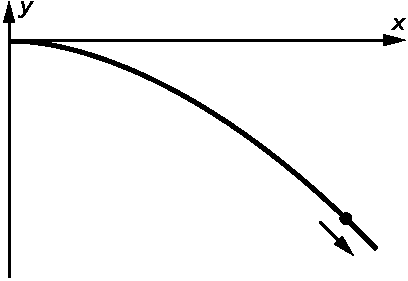
\includegraphics[width=0.7\linewidth]{fyz_fig0100.pdf}
      \caption{Parabola, již opisuje padající těleso, které má počáteční horizontální rychlost
               (\cite[s.~119]{Feynman01})}
      \label{fyz:fig0100}
    \end{figure}
    a protože při pohybu dolů je zrychlení \(-g\) konstantní, je možné vzdálenost \(y\) padajícího 
    předmětu zapsat ve tvaru
    \begin{equation}\label{fyz:eq098}
      y = -\frac{1}{2}gt^2.
    \end{equation}
    
    Jak vypadá křivka takovéhoto pohybu, tj. jaký je vztah mezi \(y\) a \(x\)? Z rovnice 
    (\ref{fyz:eq098}) můžeme vyloučit čas, neboť \(t= x/u\). Po této substituci dostaneme
    \begin{equation}\label{fyz:eq099}
      y = -\frac{g}{2u^2}x^2.
    \end{equation}
    Tento vztah mezi \(x\) a \(y\) je možné považovat za rovnici trajektorie pohybující se kuličky. 
    Vyneseme-li závislost do grafu, získáme křivku, jež se nazývá \textbf{parabola} (obr. 
    \ref{fyz:fig0100}). Jakékoli padající těleso vystřelené v libovolném směru se bude pohybovat po 
    parabole. 
  
  \section{Příklady a cvičení}
    %---------------------------------------------------------------
      % !TeX spellcheck = cs_CZ
  
Nyní si demonstrujeme užití pohybových rovnic při popisu trajektorie, libovolného bodu na 
železničním kole, které se odvaluje po kolejnici \textbf{bez} smyku. Na obrázku \ref{fyz:fig142} 
vidíme, že železniční kola jsou opatřena \emph{okolky}, která slouží jako bezpečnostní prvek proti 
vykolejení a pro hladký průjezd kolejových spojek, výhybek apod. Úlohu můžeme formulovat pro různé 
body, které mají vzdálenost od středu kola menší, větší, nebo rovnou poloměru nákolku. Otázka zní, 
jak bude jejich trajektorie rozvinutá v čase vypadat.

\begin{figure}[ht!]  %\ref{fyz:fig142}
  \centering
  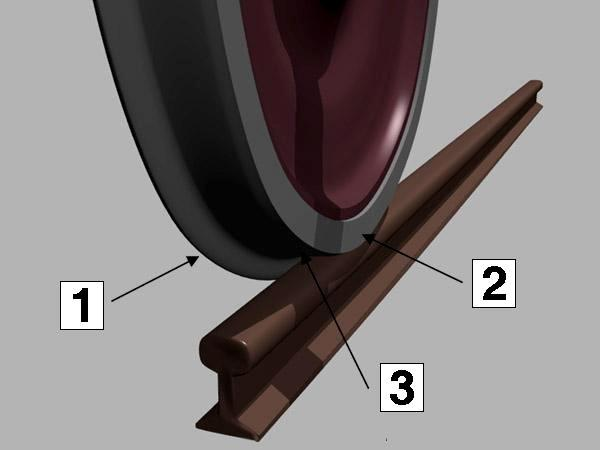
\includegraphics[width=0.5\linewidth]{fyz_fig142.jpg}
  \caption{Nákres železničního kola s částí kolejnice: \(1\ldots\text{okolek}\), \(2\ldots 
          \text{nákolek}\), \(3\ldots\text{plocha odvalování}\), kredit: \wikiOkolek. K příkladu 
          \ref{fyz:exam003}.}
  \label{fyz:fig142}
\end{figure}

\wikitextrule
\begin{example}\label{fyz:exam003}
  Kolo vagónu se valí po vodorovné kolejnici. Uvažujme bod, který je v počátečním okamžiku pod 
  středem kola ve vzdálenosti, která může být menší, rovna nebo větší než vzdálenost středu kola od 
  kolejnice.

   {\centering
    \captionsetup{type=figure}
    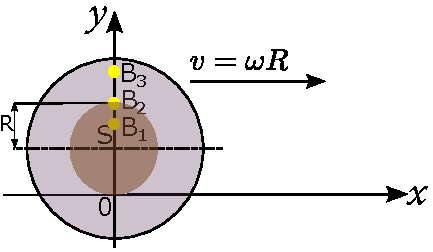
\includegraphics[width=0.6\linewidth]{fyz_fig141.pdf}
    \captionof{figure}{Kolo vagónu a tři možné polohy bodu}
    \label{fyz:fig141}
  \par}
  \vspace{0.5em}
  Určeme parametrické rovnice dráhy zvoleného bodu, složky rychlosti a její velikost, složky 
  zrychlení a jeho velikost, tečné a normálové zrychlení a poloměr křivosti dráhy. 
  \cite[p.~11]{Slavik}
  \vspace{1em}
  \newline
  \textbf{Řešení}: Obvodová rychlost v místě dotyku s kolejnicí je \(v=\omega R\), což vzhledem k 
  předpokladu o valení představuje posuvnou rychlost kola. Parametrické rovnice pro střed kola jsou pak
  \begin{subequations}\label{mech:eq_wheel_center}
    \begin{align}
      x_s &= \omega R t \\
      y_s &= R
    \end{align}
  \end{subequations}

   {\centering
    \captionsetup{type=figure}
    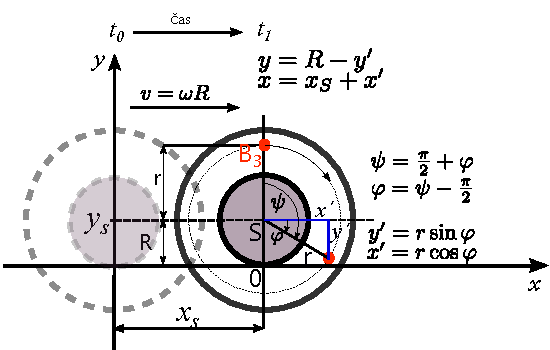
\includegraphics[width=0.9\linewidth]{fyz_fig143.pdf}
    \captionof{figure}{Náčrt pro odvození parametrických rovnic pohybu libovolně zvoleného bodu na 
               kole vagónu}
    \label{fyz:fig143}
  \par}
  \vspace{0.5em}
  Uvažovaný bod \(B_3\) na obr. \ref{fyz:fig143} je ve své nové pozici v čase \(t_1\) posunut vůči 
  středu o vzdálenost \(r\cdot\sin\omega t\) ve směru osy \(x\) a o vzdálenost \(r\cdot\cos\omega 
  t\) ve směru osy \(y\). Z obrázku \ref{fyz:fig143} lze odvodit následující rovnice pro souřadnice 
  libovolného bodu \(B\) na kole vagónu.
  
           
    \begin{itemize}
      \item ve směru osy \(x\):
      \begin{align*}
        x &= x_s + x'                        \\
        x &= x_s + r\cos(\psi-\frac{\pi}{2}) \\
        x &= x_s + r\sin\psi                 \\
        x &= \omega R t + r\sin\omega t
      \end{align*}
      \end{itemize}  


   \begin{itemize}
      \item ve směru osy \(y\): 
      \begin{align*}
        y &= y_s - y'                        \\
        y &= y_s - r\sin(\psi-\frac{\pi}{2}) \\
        y &= y_s + r\cos\psi                 \\
        y &= R + r\cos\omega t
      \end{align*}
    \end{itemize}

  takže, parametrické rovnice dráhy mají tvar \textbf{cykloidy}:
  \begin{equation*}
    x = \omega R t + r\sin\omega t  \qquad y = R + r\cos\omega t
  \end{equation*}
  \begin{itemize}
    \item Složky rychlosti:
      \begin{align*} 
       v_x &= \frac{dx}{dt} = \omega R + r\omega\cos\omega t                       \\
       v_y &= \frac{dy}{dt} = -r\omega\sin\omega t                                 \\
       v   &= \sqrt{v_x^2 + v_y^2}= \omega\sqrt{R^2 + 2Rr\cos\omega t + r^2}
      \end{align*}
    \item Složky zrychlení:
      \begin{align*}
        a_x &= \frac{dv_x}{dt} = -r\omega^2\sin\omega t                           \\
        a_y &= \frac{dv_y}{dt} = -r\omega^2\cos\omega t                           \\
        a   &= \sqrt{a_x^2 + a_y^2}= r\omega^2\sqrt{\sin^2\omega t + 
               \cos^2\omega t} = r\omega^2
      \end{align*}
      Tento výsledek je superpozicí rovnoměrného kruhového a rovnoměrného přímočarého pohybu.
    \item \textbf{Tečné zrychlení} \(a_t\) dostaneme derivací velikosti rychlosti
      \begin{equation*}
        a_t = \frac{dv}{dt} = -\cdot\frac{2Rr\omega^2\sin\omega t }{2\sqrt{R^2 + 
                2Rr\cos\omega t + r^2}}
      \end{equation*}
    \item \textbf{Normálové zrychlení} \(a_n\) získáme užitím Pythagorovy věty
      \begin{align*}
        a_n &= \sqrt{a^2 - a_t^2}                                                 \\
        a_n &= \sqrt{(r\omega^2)^2-\left(
               \frac{Rr\omega^2\sin\omega t}
                    {\sqrt{R^2 + 2Rr\cos\omega t + r^2}}\right)^2}
      \end{align*}
    \item \textbf{Poloměr křivosti} $R_0$ dostaneme ze vztahu $a_n=\frac{v^2}{R_0}$:
      \begin{equation*}
          R_0 =  \dfrac{\omega^2\cdot(R^2 + 2Rr\cos\omega t + r^2)}{\sqrt{r^2\omega^4 - 
                   \dfrac{R^2r^2\omega^4\sin^2\omega t}{R^2 + 2Rr\cos\omega t + r^2}}}
      \end{equation*}
      Poloměr křivosti není roven vzdálenosti od středu kola r: drahou bodu není kružnice, nýbrž 
      cykloida (viz obr. \ref{fyz:fig140}). Pokud bod pevně spojený s kružnicí leží na 
      jejím obvodu, pak při valení této kružnice po přímce opisuje tento bod \textbf{prostou} 
      (obecnou) cykloidu. 
  \end{itemize}
  
  \begin{align*}
    (x - \omega R t)^2            &= r^2\sin^2\omega t                          \\
    (y-R)^2                       &= r^2\cos\omega t                            \\
    (x - \omega R t)^2 + (y-R)^2  &= r^2\sin^2\omega t + r^2\cos\omega t        \\
    (x - \omega R t)^2 + (y-R)^2  &= r^2 \quad                                  \\
    \shortintertext{kde \(t = \frac{1}{\omega}\arccos\frac{y-R}{r}\)}
    \Aboxed{\left(x - R\arccos\frac{y-R}{r}\right)^2 + (y-R)^2  &= r^2}
  \end{align*}

   {\centering
    \captionsetup{type=figure}
 %   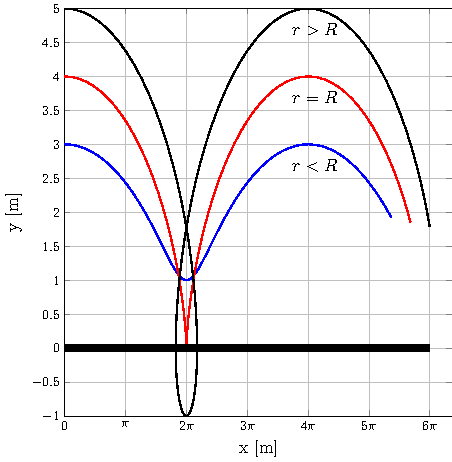
\includegraphics[width=0.8\linewidth]{fyz_fig140.pdf}
    % file: fyz_fig140.tex
% This file was created by matlab2tikz.
%
%The latest updates can be retrieved from
%  http://www.mathworks.com/matlabcentral/fileexchange/22022-matlab2tikz-matlab2tikz
%where you can also make suggestions and rate matlab2tikz.
%
\begin{tikzpicture}[scale=0.6]

\begin{axis}[%
  width=4.306in,
  height=4.528in,
  at={(0.722in,0.611in)},
  scale only axis,
  xmin=0,
  xmax=20,
  xtick={0,3.14159265358979,6.28318530717959,9.42477796076938,12.5663706143592,15.707963267949,18.8495559215388,21.9911485751286,25.1327412287183},
  xticklabels={{0},{\(\pi\)},{\(2\pi\)},{\(3\pi\)},{\(4\pi\)},{\(5\pi\)},{\(6\pi\)},{\(6\pi\)},{\(8\pi\)}},
  xlabel={\Large x [m]},
  xmajorgrids,
  ymin=-1,
  ymax=5,
  ylabel={\Large y [m]},
  ymajorgrids,
  axis background/.style={fill=white}
]
\addplot [color=blue,solid,line width=1.0pt,forget plot]
  table[row sep=crcr]{%
0	3\\
0.286333831818311	2.99544401045211\\
0.571798855564011	2.98181755588998\\
0.855534179725487	2.95924480028271\\
1.13669467377758	2.92793142610753\\
1.41445866899325	2.88816276017536\\
1.68803544547188	2.84030117373882\\
1.95667243716243	2.78478278057302\\
2.2196620892296	2.72211346311592\\
2.47634830527867	2.65286426287812\\
2.72613242569217	2.57766617712461\\
2.96847868260375	2.4972044092408\\
3.20291908180385	2.41221212517367\\
3.42905766709306	2.32346377283893\\
3.64657412822683	2.23176802536784\\
3.85522671957563	2.13796041249453\\
4.05485446290616	2.04289570722652\\
4.24537861421158	1.94744013717097\\
4.42680338122528	1.85246349148679\\
4.59921588508011	1.75883119538405\\
4.76278536646244	1.66739642438753\\
4.91776164349451	1.57899233021916\\
5.06447283539702	1.49442444913699\\
5.20332237267356	1.41446336190563\\
5.33478532106034	1.33983767228038\\
5.45940405273711	1.27122736798514\\
5.57778330424324	1.20925762467838\\
5.69058466613095	1.1544931093657\\
5.79852055456608	1.10743283516581\\
5.90234771980685	1.06850561431346\\
6.00286035071135	1.03806615083132\\
6.10088283810525	1.01639180847432\\
6.19726226294983	1.00368008339693\\
6.29286067775796	1.00004680457233\\
6.38854725158968	1.00552507836121\\
6.48519035020179	1.02006498684734\\
6.58364962351733	1.04353404268853\\
6.6847681725134	1.07571839633857\\
6.78936486690267	1.11632478463977\\
6.89822688360971	1.16498320303079\\
7.01210253403131	1.22125027702041\\
7.13169444543863	1.28461330220665\\
7.25765315865222	1.35449491602859\\
7.3905712003277	1.43025835868189\\
7.5309776838652	1.51121327526087\\
7.67933348813913	1.59662200625796\\
7.83602705797955	1.68570630910172\\
8.00137086467097	1.77765444948689\\
8.17559855872052	1.87162859788037\\
8.35886284083946	1.96677246380645\\
8.55123407053743	2.06221909834774\\
8.75269962500815	2.15709879376552\\
8.96316401414808	2.25054700825854\\
9.1824497506603	2.3417122436498\\
9.41029896731505	2.42976380422016\\
9.64637576663052	2.51389936599034\\
9.89026928156366	2.59335228748028\\
10.1414974193222	2.66739859533028\\
10.3995112541838	2.73536358113108\\
10.6637000292963	2.79662794935282\\
10.9333967218807	2.85063346035295\\
11.2078841211294	2.89688801704418\\
11.4864013634157	2.93497014887285\\
11.7681508652674	2.96453285224982\\
12.0523055909307	2.98530675243991\\
12.3380165883028	2.99710255809884\\
12.6244207245654	2.99981278609203\\
12.9106485510334	2.99341274087867\\
13.1958322255526	2.97796073953694\\
13.4791134202598	2.95359758038007\\
13.7596511426479	2.920545260005\\
14.0366293986721	2.87910495046405\\
14.3092646280711	2.82965425499148\\
14.576812844151	2.7726437672907\\
14.8385764129771	2.7085929657339\\
15.0939104101996	2.63808547988592\\
15.3422284975907	2.5617637724839\\
15.5830082657464	2.48032328533025\\
15.8157959942697	2.39450610244145\\
16.0402107860621	2.30509418819405\\
16.2559480380492	2.21290226208159\\
16.4627822167181	2.1187703750076\\
16.6605689131738	2.02355625475934\\
16.8492461589901	1.92812749041013\\
};
\node[right, align=left, text=black]
at (axis cs:11.5,2.7) {\Large \(r<R\)};
\addplot [color=red,solid,line width=1.0pt,forget plot]
  table[row sep=crcr]{%
0	4\\
0.381681731926347	3.99088802090423\\
0.761625847707474	3.96363511177995\\
1.13811056432015	3.91848960056541\\
1.50944562071406	3.85586285221506\\
1.87398767943513	3.77632552035071\\
2.23015530068212	3.68060234747763\\
2.57644335235294	3.56956556114604\\
2.911436724777	3.44422692623183\\
3.23382322516487	3.30572852575625\\
3.54240553428159	3.15533235424922\\
3.83611211639449	2.99440881848161\\
4.1140069830844	2.82442425034734\\
4.37529822195256	2.64692754567785\\
4.61934521250981	2.46353605073567\\
4.84566446349715	2.27592082498905\\
5.05393401844793	2.08579141445304\\
5.24399638934849	1.89488027434194\\
5.41585999166562	1.70492698297359\\
5.56969906766501	1.51766239076811\\
5.70585209871938	1.33479284877505\\
5.82481872107327	1.15798466043832\\
5.92725517316801	0.988848898273986\\
6.01396831601081	0.828926723811252\\
6.08590828107409	0.679675344560767\\
6.14415981271736	0.542454735970277\\
6.18993238401934	0.418515249356769\\
6.22454917608448	0.308986218731405\\
6.24943502124447	0.214865670331623\\
6.26610342001574	0.137011228626926\\
6.27614275011447	0.0761323016626385\\
6.28120179319199	0.0327836169486335\\
6.28297471117087	0.00736016679385365\\
6.28318560907687	9.36091446517295e-05\\
6.28357282503002	0.0110501567224259\\
6.28587309054397	0.0401299736946852\\
6.29180570546478	0.0870680853770696\\
6.30305687174664	0.151436792677134\\
6.32126432881491	0.232649569279539\\
6.34800243051873	0.329966406061573\\
6.38476779965164	0.442500554040812\\
6.432965690756	0.569226604413309\\
6.49389718547292	0.708989832057179\\
6.56874733711361	0.860516717363772\\
6.65857437247832	1.02242655052173\\
6.76430004931591	1.19324401251592\\
6.88670125728648	1.37141261820345\\
7.02640293895904	1.55530889897378\\
7.18387239534787	1.74325719576073\\
7.35941502787546	1.9335449276129\\
7.55317155556114	2.12443819669547\\
7.7651167327923	2.31419758753104\\
7.99505957936188	2.50109401651708\\
8.24264512067606	2.6834244872996\\
8.50735762227529	2.85952760844031\\
8.78852528919594	3.02779873198067\\
9.08532638735196	3.18670457496056\\
9.39679673115867	3.33479719066056\\
9.72183846917169	3.47072716226216\\
10.0592300876863	3.59325589870564\\
10.4076375411449	3.7012669207059\\
10.765626407932	3.79377603408835\\
11.1316749607943	3.8699402977457\\
11.5041880327875	3.92906570449965\\
11.8815115524038	3.97061350487982\\
12.2619476154377	3.99420511619768\\
12.6437699562527	3.99962557218406\\
13.0252396774784	3.98682548175734\\
13.4046210948066	3.95592147907389\\
13.7801975525107	3.90719516076014\\
14.1502870655765	3.84109052001\\
14.5132576459148	3.75820990092809\\
14.8675421730024	3.65930850998295\\
15.2116526734519	3.54528753458141\\
15.5441938793939	3.4171859314678\\
15.8638759421286	3.27617095977184\\
16.1695261852006	3.1235275449678\\
16.4600997898016	2.96064657066049\\
16.7346893151381	2.7890122048829\\
16.9925329670126	2.6101883763881\\
17.2330215392765	2.42580452416318\\
17.455703964904	2.23754075001519\\
17.6602914261051	2.04711250951867\\
17.8466599860274	1.85625498082027\\
};
\node[right, align=left, text=black]
at (axis cs:11.5,3.7) {\Large \(r=R\)};
\addplot [color=black,solid,line width=1.0pt,forget plot]
  table[row sep=crcr]{%
0	5\\
0.477029632034383	4.98633203135634\\
0.951452839850936	4.94545266766993\\
1.42068694891481	4.87773440084812\\
1.88219656765054	4.7837942783226\\
2.33351668987702	4.66448828052607\\
2.77227515589235	4.52090352121645\\
3.19621426754345	4.35434834171905\\
3.6032113603244	4.16634038934775\\
3.99129814505107	3.95859278863437\\
4.35867864287101	3.73299853137383\\
4.70374555018523	3.49161322772241\\
5.02509488436496	3.236636375521\\
5.32153877681206	2.97039131851678\\
5.5921162967928	2.69530407610351\\
5.83610220741866	2.41388123748358\\
6.05301357398969	2.12868712167956\\
6.2426141644854	1.84232041151291\\
6.40491660210596	1.55739047446038\\
6.54018225024991	1.27649358615216\\
6.64891883097633	1.00218927316258\\
6.73187579865202	0.736976990657473\\
6.79003751093899	0.48327334741098\\
6.82461425934806	0.243390085716878\\
6.83703124108784	0.0195130168411501\\
6.82891557269761	-0.186317896044585\\
6.80208146379544	-0.372227125964847\\
6.75851368603802	-0.536520671902893\\
6.70034948792286	-0.677701494502565\\
6.62985912022463	-0.794483157059612\\
6.54942514951759	-0.885801547506042\\
6.46152074827874	-0.95082457457705\\
6.36868715939191	-0.98895974980922\\
6.27351054039578	-0.999859586283022\\
6.17859839847037	-0.983424764916361\\
6.08655583088616	-0.939805039457972\\
5.99996178741223	-0.869397871934396\\
5.92134557097988	-0.772844810984298\\
5.85316379072715	-0.651025646080691\\
5.79777797742774	-0.50505039090764\\
5.75743306527198	-0.336249168938781\\
5.73423693607337	-0.146160093380037\\
5.73014121229362	0.0634847480857685\\
5.74692347389951	0.290775076045659\\
5.78617106109144	0.533639825782596\\
5.84926661049269	0.789866018773876\\
5.93737545659341	1.05711892730517\\
6.05143501324711	1.33296334846066\\
6.19214623197522	1.6148857936411\\
6.35996721491147	1.90031739141935\\
6.55510904058485	2.18665729504321\\
6.77753384057645	2.47129638129656\\
7.02695514457569	2.75164102477562\\
7.30284049069182	3.02513673094941\\
7.60441627723552	3.28929141266047\\
7.93067481176137	3.54169809797101\\
8.28038349314025	3.78005686244085\\
8.65209604299518	4.00219578599084\\
9.04416568415957	4.20609074339324\\
9.45476014607637	4.38988384805846\\
9.8818783604091	4.55190038105885\\
10.3233686947346	4.69066405113253\\
10.776948558173	4.80491044661855\\
11.2402252003075	4.89359855674947\\
11.7107175138769	4.95592025731973\\
12.1858786425726	4.99130767429652\\
12.6631191879399	4.9994383582761\\
13.1398308039234	4.980238222636\\
13.6134099640606	4.93388221861083\\
14.0812816847616	4.86079274114022\\
14.5409229885052	4.76163578001499\\
14.9898858931575	4.63731485139214\\
15.4258197179337	4.48896276497443\\
15.8464925027528	4.31793130187211\\
16.2498113458106	4.1257788972017\\
16.6338414740577	3.91425643965775\\
16.9968238728105	3.6852913174517\\
17.3371913138569	3.44096985599074\\
17.6535826360064	3.18351830732435\\
17.944855147963	2.91528256458215\\
18.2100950405038	2.63870678624476\\
18.4486257130899	2.35631112502279\\
18.6600139390365	2.07066876427801\\
18.8440738130648	1.7843824712304\\
};
\node[right, align=left, text=black]
at (axis cs:11.5,4.7) {\Large\(r>R\)};
\addplot [color=black,solid,line width=6.0pt,forget plot]
  table[row sep=crcr]{%
0	0\\
0.477029632034383	0\\
0.951452839850936	0\\
1.42068694891481	0\\
1.88219656765054	0\\
2.33351668987702	0\\
2.77227515589235	0\\
3.19621426754345	0\\
3.6032113603244	0\\
3.99129814505107	0\\
4.35867864287101	0\\
4.70374555018523	0\\
5.02509488436496	0\\
5.32153877681206	0\\
5.5921162967928	0\\
5.83610220741866	0\\
6.05301357398969	0\\
6.2426141644854	0\\
6.40491660210596	0\\
6.54018225024991	0\\
6.64891883097633	0\\
6.73187579865202	0\\
6.79003751093899	0\\
6.82461425934806	0\\
6.83703124108784	0\\
6.82891557269761	0\\
6.80208146379544	0\\
6.75851368603802	0\\
6.70034948792286	0\\
6.62985912022463	0\\
6.54942514951759	0\\
6.46152074827874	0\\
6.36868715939191	0\\
6.27351054039578	0\\
6.17859839847037	0\\
6.08655583088616	0\\
5.99996178741223	0\\
5.92134557097988	0\\
5.85316379072715	0\\
5.79777797742774	0\\
5.75743306527198	0\\
5.73423693607337	0\\
5.73014121229362	0\\
5.74692347389951	0\\
5.78617106109144	0\\
5.84926661049269	0\\
5.93737545659341	0\\
6.05143501324711	0\\
6.19214623197522	0\\
6.35996721491147	0\\
6.55510904058485	0\\
6.77753384057645	0\\
7.02695514457569	0\\
7.30284049069182	0\\
7.60441627723552	0\\
7.93067481176137	0\\
8.28038349314025	0\\
8.65209604299518	0\\
9.04416568415957	0\\
9.45476014607637	0\\
9.8818783604091	0\\
10.3233686947346	0\\
10.776948558173	0\\
11.2402252003075	0\\
11.7107175138769	0\\
12.1858786425726	0\\
12.6631191879399	0\\
13.1398308039234	0\\
13.6134099640606	0\\
14.0812816847616	0\\
14.5409229885052	0\\
14.9898858931575	0\\
15.4258197179337	0\\
15.8464925027528	0\\
16.2498113458106	0\\
16.6338414740577	0\\
16.9968238728105	0\\
17.3371913138569	0\\
17.6535826360064	0\\
17.944855147963	0\\
18.2100950405038	0\\
18.4486257130899	0\\
18.6600139390365	0\\
18.8440738130648	0\\
};

\addplot [color=black,solid,line width=6.0pt,forget plot]
  table[row sep=crcr]{%
0	0\\
18.8440738130648	0\\
};
\end{axis}
\end{tikzpicture}%
    \captionof{figure}{Cykloida: pro $B_2\ldots r=R$ je cykloida prostá; $B_3\ldots r>R$
              cykloida prodloužená; $B_1\ldots r<R$ cykloida zkrácená; \texttt{[cykloida.m]} }
    \label{fyz:fig140}
    \par}       
    \vspace{1em}
   
   Z obrázku \ref{fyz:fig140} je také patrné, že pokud bod pevně spojený s kutálející se kružnicí 
   neleží na obvodu této kružnice, ale jeho vzdálenost od středu kružnice o poloměru \(R\)  je 
   \(r\) , pak pro \(r<R\) získáme \textbf{cykloidu zkrácenou} a pro \(r>R\)  \textbf{cykloidu 
   prodlouženou}.
      
%---------------------------------------------------------------
\lstinputlisting[language=Matlab]{../src/FYZ/matlab/cicloid.m}
\begin{lstlisting}[caption= Výpočet křivky cykloidy pro pro tři různé body.]
\end{lstlisting}
%---------------------------------------------------------------

%    %---------------------------------------------------------------
%      \tikzexternaldisable
%      % !TeX spellcheck = cs_CZ

% note:
% ~~~~~~
% This figure uses expl3 package for coordinate calculating !!!
%\usepackage{expl3}                     % fpeval
%\ExplSyntaxOn
%\cs_set_eq:NN \fpeval \fp_eval:n
%\ExplSyntaxOff
%-------------------------------------------------------------------------------------------------
\def\xmin{0}
\def\xmax{8.5}
\def\ymin{-0.75}
\def\ymax{+2}
\def\zero{0}
\def\R{0.5}
\def\r{0.5}
\def\omega{4/3.14}
\def\angle{360}

{\centering
 \captionsetup{type=figure}
\begin{animateinline}
 [autoplay,
  palindrome,
  begin={
    \begin{tikzpicture}
      \useasboundingbox (\xmin,\ymin) rectangle (\xmax,\ymax);

      \draw [step=1cm, black!40!white, very thin] (\xmin cm,\ymin cm) grid (\xmax cm,\ymax cm);
      \draw [red, thick,  domain=0:6*pi, samples=100] 
        plot ({\omega*\R*\x + \r*sin(deg(\omega*\x))}, {\R+\r*cos(deg(\omega*\x))} );
        
      \draw [Mahogany, thick,  domain=0:6*pi, samples=100] 
        plot ({\omega*\R*\x + 1.5*\r*sin(deg(\omega*\x))}, {\R+1.5*\r*cos(deg(\omega*\x))} );
        
      \draw [orange, thick,  domain=0:6*pi, samples=100] 
        plot ({\omega*\R*\x + 0.4*\r*sin(deg(\omega*\x))}, {\R+0.4*\r*cos(deg(\omega*\x))} );
        
      \draw[black, thick] (\xmin cm,\ymin cm) rectangle (\xmax cm,\ymax cm);
    
      \draw [Sepia,line width=0.5mm] (\xmin,0) -- (\xmax,0);
        \foreach \x/\xtext in {1/1,2/2,3/3,4/4,5/5,6/6,7/7,8/8}
          \draw (\x cm,-3pt) -- (\x cm,2pt) node[below, yshift=-1mm, fill=white] {\xtext};
        },
  end={\end{tikzpicture}}
]{5}
  \multiframe{40}{nstep=0.1+20}{% 
    % wheel
    \filldraw[fill=black!40!white, draw=black, opacity=0.2] 
      (\nstep/57.295/3.14*2, \R cm) circle (\R cm);
    %point 1
    \filldraw[fill=red!40!white, draw=black] (\fpeval{\omega*\R*\nstep/57.295 + 
       1.0*\r*sin(deg(\omega*\nstep))},\fpeval{\R+1.0*\r*cos(deg(\omega*\nstep))}) circle (0.5 mm);
    %point 2
    \filldraw[fill=red!40!white, draw=black] (\fpeval{\omega*\R*\nstep/57.295 + 
       1.5*\r*sin(deg(\omega*\nstep))},\fpeval{\R+1.5*\r*cos(deg(\omega*\nstep))}) circle (0.5 mm);
    %point 3
    \filldraw[fill=red!40!white, draw=black] (\fpeval{\omega*\R*\nstep/57.295 + 
       0.4*\r*sin(deg(\omega*\nstep))},\fpeval{\R+0.4*\r*cos(deg(\omega*\nstep))}) circle (0.5 mm);
}
\end{animateinline}
\captionof{figure}{Animace parametrických rovnic pohybu libovolně zvoleného bodu na kole}
\label{fyz:fig144}
\par}
%      \tikzexternalenable
%    %---------------------------------------------------------------
    
\end{example}
\wikitextrule

    %---------------------------------------------------------------

%} %tikzset
%---------------------------------------------------------------------------------------------------